\documentclass[12pt,a4paper]{article}
\usepackage{cmap} % Makes the PDF copiable. See http://tex.stackexchange.com/a/64198/25761
\usepackage[T1]{fontenc}
\usepackage[brazil]{babel}
\usepackage[utf8]{inputenc}
\usepackage{amsmath}
\usepackage{amsfonts}
\usepackage{amssymb}
\usepackage{amsthm}
\usepackage{textcomp} % \degree
\usepackage{gensymb} % \degree
\usepackage[usenames,svgnames,dvipsnames]{xcolor}
\usepackage{hyperref}
\usepackage{graphicx}
\usepackage[margin=2cm]{geometry}

\hypersetup{
    colorlinks = true,
    allcolors = {blue}
}

\newcommand*\diff{\mathop{}\!\mathrm{d}}
\newcommand*\sen{\operatorname{sen}}
\newcommand*\senh{\operatorname{senh}}

\newcommand*\R{\mathbb{R}}

\newcommand*\prova{Prova II}
\newcommand*\turma{TADS121-01C}
\newcommand*\disciplina{CDI0001}
\newcommand*\eu{Helder G. G. de Lima}
\newcommand*\data{07/05/2016}

\author{\eu}
\title{\prova - \disciplina}
\date{\data}

\begin{document}
\thispagestyle{empty}
\newgeometry{margin=2cm,bottom=0.5cm}
\begin{center}

\includegraphics[width=9.0cm]{marca}
\noindent\begin{tabular}{l c c r}
  \textbf{\disciplina (\turma)}
& \textbf{\prova}
& \textbf{\data}
\end{tabular}
\\ Prof. \eu\footnote{
Este é um material de acesso livre distribuído sob os termos da licença \href{https://creativecommons.org/licenses/by-sa/4.0/deed.pt_BR}{Creative Commons BY-SA 4.0}.}
\end{center}

\noindent Nome do(a) aluno(a): \rule{13cm}{0.01cm}

%\section*{Instruções}
\begin{center}\fbox{
\begin{minipage}{14cm}

{\footnotesize
\begin{itemize}
\renewcommand{\theenumi}{\Roman{enumi}}
\item Identifique-se em todas as folhas.
\item Mantenha o celular e os demais equipamentos eletrônicos desligados durante a prova.
\item Anule uma das 6 questões (apenas 5 serão corrigidas). \textsc{\textbf{Questão anulada:}} \framebox(30,12){}
\end{itemize}
}

\end{minipage}
}
\end{center}


%\section*{Questões}

\begin{enumerate}
\item (2,0) Seja $g: \R \setminus \{-3, 3\} \to \R$ dada por $g(x) = \dfrac{x^2}{x^2-9}$.
\begin{enumerate}
\item (1,0) Utilize a definição de derivada para obter uma fórmula para $g^\prime(x)$.
\item (1,0) Qual é a equação da reta tangente ao gráfico de $g$ no ponto de abcissa $-1$?
\end{enumerate}

\item (2,0) Determine para que valores das constantes $b$ e $c$ a função
\[ q(x) = \ln\left(\frac{b}{x}\right) + \frac{c}{\ln(x)}\]
satisfaz $q^\prime(e) = 1 = q(e)$, sendo $e$ a constante de Euler.


\item (2,0) Suponha que $h: [-1,1] \to [0, \pi]$ seja definida por $h(x) = \arccos(x)$.
\begin{enumerate}
\item (1,5) Deduza $\frac{ \diff{h} }{\diff{x} }(x)$ (dica: defina $h$ implicitamente por alguma equação).
\item (0,5) Calcule $q'(0)$, sendo $q:[-2,2] \to \mathbb{R}$ definida por $q(x) = 4h(x/2)$.
\end{enumerate}



\item (2,0) Considere a função $f: \R \to \R$ definida por $f(x) = \senh(2x) + \cosh(2x)$.
\begin{enumerate}
\item (1,0) Determine a equação da reta normal ao gráfico de $f$ no ponto $P = (0, f(0))$.
\item (1,0) Obtenha uma fórmula para $f^{(n)}(x)$ (a $n$-ésima derivada de $f$).
\end{enumerate}

\item (2,0) Utilize uma aproximação por diferenciais (aproximação linear) para estimar o volume de material necessário para fazer uma bola com espessura de $0,1 cm$ e raio interno de $5 cm$.

\item (2,0) Ao andar por uma calçada, você está se afastando de uma luminária de $2,7m$ de altura a uma velocidade de $1,5 m/s$. Assumindo que você tenha $1,8m$ de altura, utilize o que aprendeu sobre derivadas para determinar com que velocidade o comprimento da sua sombra no chão aumenta conforme você se afasta da luminária.
\end{enumerate}

\begin{center}
BOA PROVA!
\end{center}

\newpage
\restoregeometry
\section*{Respostas e observações}
\begin{enumerate}
\item \begin{enumerate}
\item Pela definição de derivada,
\begin{align*}
g^\prime(x)
& = \lim_{h \to 0} \frac{\frac{(x+h)^2}{(x+h)^2 - 9} - \frac{x^2}{x^2 - 9}}{h}
= \lim_{h \to 0} \frac{(x^2 - 9) (x+h)^2 - x^2((x+h)^2 - 9)}{h ((x+h)^2 - 9)(x^2 - 9)} \\
& = \lim_{h \to 0} \frac{-9(x+h)^2 + 9x^2}{h((x+h)^2 - 9)(x^2 - 9)}
  = \lim_{h \to 0} 9 \frac{-(x^2 +2xh + h^2) + x^2}{h((x+h)^2 - 9)(x^2 - 9)} \\
& = \lim_{h \to 0} 9 \frac{-2xh -h^2}{h((x+h)^2 - 9)(x^2 - 9)}
  = \lim_{h \to 0} 9 \frac{-2x -h}{((x+h)^2 - 9)(x^2 - 9)} \\
& = \dfrac{-18x}{(x^2- 9)^2}
  = \dfrac{-18x}{x^4 - 18x^2 + 81}.
\end{align*}

\item Como $g(-1) = -\frac{1}{8}$ e pelo item anterior $g^\prime(-1) = \frac{-18(-1)}{(1-9)^2} = \frac{18}{64} = \frac{9}{32}$, tem-se
\[
y = -\frac{1}{8} + \frac{9}{32}(x + 1) = \frac{9}{32}x + \frac{5}{32} = 0,28x + 0,16.
\]
\end{enumerate}
\item Pelas propriedades do logaritmo, tem-se $q(x) = \ln(b) - \ln(x) + \frac{c}{\ln(x)}$. Então
\[
q(e) = 1
\Leftrightarrow
\ln(b) - \ln({e}) + \frac{c}{\ln(e)} = 1
\Leftrightarrow
\ln(b) - 1 + c = 1
\Leftrightarrow
\ln(b) = 2 - c.
\]
Por outro lado,
\[
q^\prime(x)
= 0 - \frac{1}{x} + c \frac{-1}{\ln^2(x)}\frac{1}{x}
= - \frac{1}{x} - \frac{c}{x \ln^2(x)},
\]
e em particular,
\[
q^\prime(e)
= - \frac{1}{e} - \frac{c}{e \ln^2(e)}
= - \frac{1}{e} - \frac{c}{e} = - \frac{1+c}{e}.
\]
Assim, para que $q^\prime(e) = 1$ deve ocorrer $- \frac{1+c}{e} = 1$  e portanto $c = -e - 1$. Consequentemente, $\ln(b) = 2-(-e-1) = 3 + e$ e resulta que $b = e^{(3+e)}$.

\item
\begin{enumerate}
\item Seja $y = h(x) = \arccos(x)$. Então, por definição, $\cos(y) = x$ e derivando ambos os membros obtém-se: $\frac{ \diff{} }{ \diff{x} } \cos(y) = \frac{ \diff{x} }{ \diff{x} }$, ou seja, $-\sen(y)\frac{ \diff{y} }{ \diff{x} }  = 1$. Assim,
\[
h^\prime(x)
= \frac{ \diff{y} }{ \diff{x} }
= \frac{-1}{ \sen(y) }
= \frac{-1}{ \sqrt{ 1- \cos^2(y) } }
= \frac{-1}{ \sqrt{ 1- x^2 } }.
\]

\item Se $q(x) = 4h\left(\frac{x}{2}\right)$, então $q^\prime(x) = 4 h^\prime\left(\frac{x}{2}\right) \cdot \frac{1}{2} = \frac{-2}{ \sqrt{ 1 - \left(\frac{x}{2}\right)^2 } }$. Em particular, para $x = 0$, tem-se $q^\prime(0) = \frac{-2}{ \sqrt{ 1 - 0^2 } } = -2$.
\end{enumerate}
\item
\begin{enumerate}
\item Considerando que
\[
f(x) = \senh(2x) + \cosh(2x) = \frac{e^{2x} + e^{-2x}}{2} + \frac{e^{2x} - e^{-2x}}{2} = e^{2x},
\]
resulta que $f^\prime(x) = (e^{2x})^\prime = 2e^{2x}$, e em particular tem-se $f^\prime(0) = 2 e^{0} = 2$. Como este é o coeficiente angular da reta tangente ao gráfico de $f$ em $(0,f(0))$, e o coeficiente angular $m_n$ de qualquer reta ortogonal a esta deve satisfazer $m_n \cdot 2 = -1$, tem-se $m_n = -\frac{1}{2}$. Mas $f(0) = e^{2 \cdot 0} = 1$, então a reta normal ao gráfico de $f$ em $(0,1)$ é
\[
y = f(0) + f^\prime(0)(x-0) = 1 -\frac{1}{2}(x-0),
\]
isto é, $y = -\frac{x}{2} + 1$.
\item Pelo item anterior, $f^\prime(x) = 2e^{2x}$, então
\[
f^{\prime\prime}(x) = (2e^{2x})^\prime = 2 \cdot (2e^{2x}) = 2^2e^{2x}.
\]
De forma análoga,
\[
f^{(3)}(x) = (2^2e^{2x})^\prime = 2^2 \cdot (2e^{2x}) = 2^3e^{2x}
\]
e
\[
f^{(4)}(x) = (2^3e^{2x})^\prime = 2^3 \cdot (2e^{2x}) = 2^4e^{2x}.
\]
Como a cada etapa, a regra da cadeia faz com que o expoente de $2$ aumente em uma unidade, e ele é sempre igual ao número de vezes que a função foi derivada, conclui-se que $f^{(n)}(x) = 2^n e^{2x}$, para todo $n \in \mathbb{N}^*$.
\end{enumerate}

\item O volume de uma esfera é dado em função de seu raio $r$ pela função $V(r) = \frac{4}{3}\pi r^3$, cuja derivada é $V^\prime(r) = 4 \pi r^2$. Então, pode-se usar uma aproximação linear para estimar que $V(5,1) \approx V(5) + V^\prime(5)( 5,1 - 5,0 )$, ou ainda, que
\[
\Delta V
= V(5,1) - V(5)
\approx V^\prime(5)( 5,1 - 5,0 )
= 4 \pi 5^2 \cdot 0,1
= 10 \pi.
\]
Assim, são necessários aproximadamente $10 \pi cm^3 \approx 31,42 cm^3$ de material para fazer a bola com as dimensões especificadas. Apenas para comparação, o volume exato é:
\[
\Delta V
= V(5,1) - V(5)
= \frac{4}{3}\pi (5 +1/10)^3 - \frac{4}{3}\pi 5^3
= \frac{7651 \pi}{750}
\approx 32,05 cm^3.
\]


\item Seja $s$ o tamanho da sombra e $x$ a distância até a luminária, como na figura a seguir:
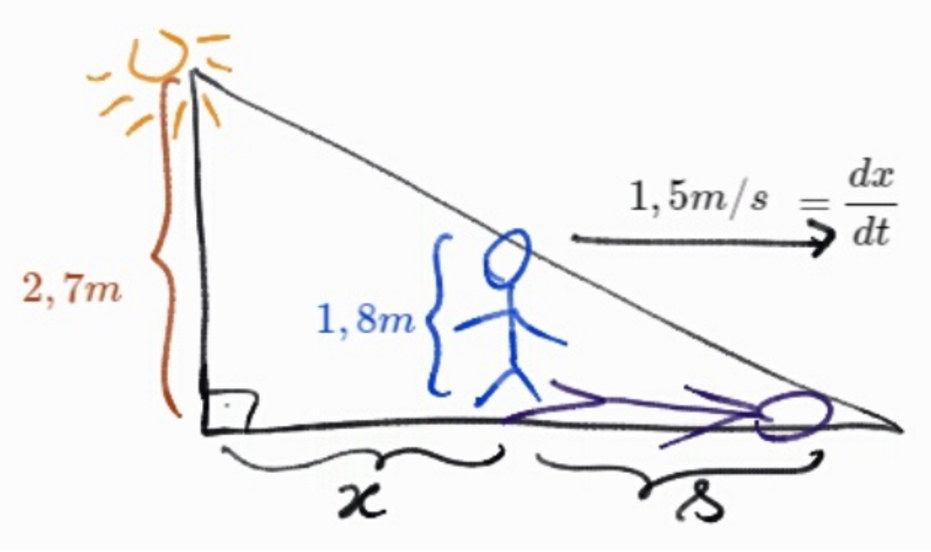
\includegraphics[width=8.0cm]{img/prova-2-tads-sombra}

Então, por semelhança de triângulos, tem-se $\frac{s}{1,8} = \frac{x+s}{2,7}$. Derivando ambos os membros em relação a $t$, obtém-se $\frac{1}{1,8}\frac{\diff{s}}{\diff{t}} = \frac{1}{2,7} \left( \frac{\diff{x}}{\diff{t}} + \frac{\diff{s}}{\diff{t}} \right)$, e como $\frac{\diff{x}}{\diff{t}} = 1,5$, conclui-se que:
\[
\frac{2,7}{1,8}\frac{\diff{s}}{\diff{t}} = 1,5 + \frac{\diff{s}}{\diff{t}}
\Leftrightarrow
\frac{3}{2}\frac{\diff{s}}{\diff{t}} -\frac{\diff{s}}{\diff{t}} = 1,5
\Leftrightarrow
\frac{1}{2}\frac{\diff{s}}{\diff{t}} = 1,5
\Leftrightarrow
\frac{\diff{s}}{\diff{t}} = 3.
\]
Assim, a sombra aumenta a uma taxa de $3m/s$.
\end{enumerate}
\end{document}
